% ============================================================
% Artigo do Projeto de Curso II no modelo IEEE Access.
% Estrutura do Apêndice L do Regulamento de Projeto de Curso: resumo e abstract (até 200 palavras),
% introdução, fundamentação teórica, metodologia, análise dos resultados, considerações finais e referências.
% Versão condensada da dissertação (docs/main.tex); os capítulos da dissertação não são alterados.
% Compilar a partir desta pasta: tectonic -X compile artigo.tex  (figuras e .bib vêm de ../)
% ============================================================
\documentclass{ieeeaccess}

\usepackage[T1]{fontenc}
\usepackage[utf8]{inputenc}
\usepackage[brazil]{babel}
\usepackage{cite}
\usepackage{amsmath,amssymb}
\usepackage{booktabs}
\usepackage{graphicx}
\usepackage{url}
\graphicspath{{../imagens/}{imagens/}}
\setlength{\emergencystretch}{3em}
\sloppy
\hyphenation{Pro-me-theus Sys-stat}

\begin{document}
\newlength{\xfigwd}  % usado pela legenda da classe ieeeaccess
\setlength{\xfigwd}{\columnwidth}

\history{Projeto de Curso II, Instituto Federal do Paraná, 2026.}
\doi{10.1109/ACCESS.2026.DOI}

\title{Monitoramento de Funções Virtualizadas de Redes: Um Estudo Comparativo entre Ferramentas de Extração de Comportamento}

\author{
\uppercase{João Pedro dos Santos Henrique Plinta}\authorrefmark{1}, and
\uppercase{Rafael Correia Alves}\authorrefmark{1}}

\address[1]{Instituto Federal do Paraná, Campus Pinhais, Pinhais, PR, Brasil}

\tfootnote{Orientador: Prof. Guilherme Werneck de Oliveira.}

\markboth
{Plinta e Alves: Monitoramento de Funções Virtualizadas de Redes}
{Plinta e Alves: Monitoramento de Funções Virtualizadas de Redes}

\corresp{Autor correspondente: João Pedro dos Santos Henrique Plinta (e-mail: joaopedrohenriqueplinta@gmail.com).}

\begin{abstract}
Network Functions Virtualization (NFV) requires continuous monitoring, but the collector runs on the same host as the monitored function and competes with it for resources. This work compares the cost of four approaches to monitoring a simplified Web Application Firewall (WAF): eBPF (libbpf with CO-RE), Sysstat, Prometheus and the Docker API. Each collector was evaluated at four message volumes (100 thousand to 2 million), with 30 repetitions per combination (480 runs). The primary metric was the observer response time (UDP RTT), complemented by CPU and memory usage, with 95\% confidence intervals. eBPF showed the lowest response time at every volume, about 13\% below Sysstat, 15\% below Prometheus and 80\% below the Docker API, with statistically significant differences; the gap to Sysstat and Prometheus is moderate in magnitude. Sysstat had the lowest memory footprint and the Docker API the highest. A complementary run, in which the WAF inspected every message, preserved the ranking of the tools.
\end{abstract}

\begin{keywords}
eBPF; network monitoring; NFV; overhead; Docker.
\end{keywords}

\titlepgskip=-15pt

\maketitle

\noindent\textbf{\textit{Resumo}}---A virtualização de funções de rede (NFV) exige monitoramento contínuo, mas o coletor executa no mesmo \textit{host} da função monitorada e compete com ela por recursos. Este trabalho compara o custo de quatro abordagens de monitoramento de um \textit{Web Application Firewall} (WAF) simplificado: eBPF (libbpf com CO-RE), Sysstat, Prometheus e API do Docker. Cada coletor foi avaliado em quatro volumes de mensagens (100 mil a 2 milhões), com 30 repetições por combinação (480 execuções). A métrica primária foi o tempo de resposta do observador (RTT UDP), complementada por CPU e memória, com intervalos de confiança de 95\%. O eBPF teve o menor tempo de resposta em todos os volumes, cerca de 13\% abaixo do Sysstat, 15\% abaixo do Prometheus e 80\% abaixo da API do Docker, com diferenças significativas; a diferença para Sysstat e Prometheus é de magnitude moderada. O Sysstat teve o menor consumo de memória e a API do Docker, o maior. Uma coleta complementar, com o WAF inspecionando todas as mensagens, preservou a ordem entre as ferramentas.

\noindent\textbf{\textit{Palavras-chave}}---eBPF; monitoramento de redes; NFV; sobrecarga; Docker.

\section{Introdução}
\label{sec:intro}
A Virtualização de Funções de Rede (NFV) desacopla as funções de rede do \textit{hardware}, e as funções virtualizadas (VNFs) passam a executar como \textit{software} em servidores comuns, com ganho de flexibilidade e redução de custos \cite{mijumbi2016,oliveira2026-sbrc}. Para que essa flexibilidade se mantenha, as VNFs precisam ser monitoradas de forma contínua, por métricas como consumo de CPU e memória, latência e vazão \cite{rfc6390}. O observador, porém, executa co-localizado à VNF e compartilha seus núcleos e sua memória; um coletor que consuma recursos em excesso degrada o serviço que deveria apenas observar \cite{10.1145/3397022}.

O \textbf{problema} investigado é: quais as diferenças práticas de desempenho entre eBPF \cite{gregg_bpf_2019}, Sysstat \cite{godard2024sysstat}, Prometheus \cite{turnbull_prometheus_2018} e a API do Docker, quando aplicados ao monitoramento de uma VNF, e qual delas oferece a menor sobrecarga. A \textbf{hipótese} é que o eBPF, por operar no \textit{kernel}, apresente o menor tempo de resposta na coleta, em relação às demais, que operam no espaço de usuário. O \textbf{objetivo} é medir e comparar o tempo de resposta e o consumo de recursos das quatro abordagens, com intervalos de confiança de 95\%. A \textbf{metodologia} é experimental: quatro pilhas idênticas de contêineres, em que só o coletor muda, quatro volumes de mensagens e 30 repetições por combinação.

O restante do artigo está organizado assim: a Seção~\ref{sec:fund} apresenta os conceitos e as quatro abordagens; a Seção~\ref{sec:met} descreve o experimento; a Seção~\ref{sec:res} analisa os resultados; e a Seção~\ref{sec:conc} traz as considerações finais.

\section{Fundamentação Teórica}
\label{sec:fund}
Em ambientes NFV, o monitoramento alimenta a orquestração, a detecção de falhas e o dimensionamento das VNFs \cite{usman_observability_2022}. As quatro abordagens comparadas diferem sobretudo no ponto em que a informação é obtida.

O \textbf{eBPF} permite executar programas verificados no \textit{kernel}, ligados a eventos como as sondas \textit{kprobes} \cite{gregg_bpf_2019,linux_bpf_docs}. Neste trabalho, o coletor usa libbpf com CO-RE e acumula contadores em mapas do \textit{kernel}, de modo que a resposta ao observador é uma leitura de memória. O \textbf{Sysstat} lê periodicamente os arquivos de \texttt{/proc}, e o \textbf{Prometheus} faz o mesmo e acrescenta um servidor HTTP para exposição das métricas \cite{godard2024sysstat,turnbull_prometheus_2018}. A \textbf{API do Docker} obtém CPU e memória dos grupos de controle (\textit{cgroups}) do \textit{kernel}, mas por consulta ao \textit{daemon} do Docker, que lê os \textit{cgroups} e serializa a resposta \cite{kernel_cgroup_v2,docker_runmetrics}.

\section{Metodologia}
\label{sec:met}
\subsection{Topologia e carga}
A topologia é igual nas quatro pilhas: um cliente envia cargas ao WAF (TCP, porta 8080), que as inspeciona em busca de injeção SQL, XSS, \textit{path traversal}, execução remota de comandos e \textit{null byte}; o observador responde, por UDP (porta 9999), a sondas enviadas a cada segundo, e o tempo de ida e volta dessa sonda (RTT UDP) é a métrica primária. Cada coletor roda em contêineres na mesma máquina (AMD Ryzen 5 5500, 16 GB, Ubuntu 26.04, \textit{kernel} 7.0, Docker 29.8). O código e os dados estão públicos\footnote{\url{https://github.com/joaopedroplinta/vnf-monitoring-benchmark}}, e os resultados das 480 execuções podem ser explorados em um painel interativo\footnote{\url{https://vnf-lab.up.railway.app}}. A Figura~\ref{fig:c4} resume a topologia.

\begin{figure*}[t]
\centering
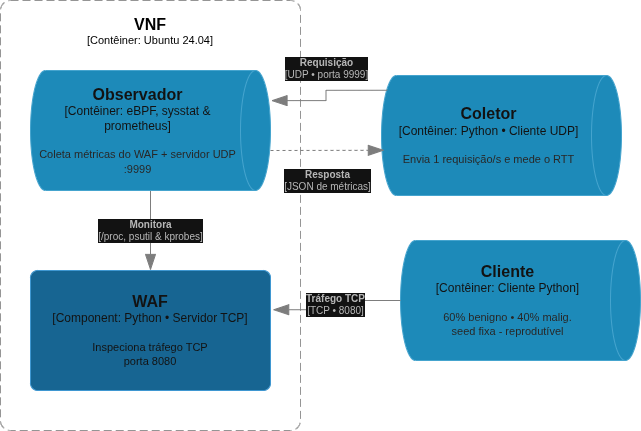
\includegraphics[width=0.6\textwidth]{C4model.drawio.png}
\caption{Diagrama de contêineres (C4, nível 2) da topologia experimental.}
\label{fig:c4}
\end{figure*}

\subsection{Protocolo e análise estatística}
O volume de mensagens $N$ assume os níveis 100 mil, 500 mil, 1 milhão e 2 milhões, e a janela de coleta dura $\lfloor N/15\,000\rfloor + 20$ s. Cada combinação de coletor e volume foi repetida 30 vezes, totalizando 480 execuções. Os resultados são reportados como média $\pm$ IC95\% (distribuição $t$ de Student); dois intervalos que não se sobrepõem são tomados como evidência de diferença ao nível $\alpha=0{,}05$. Além do RTT, mediram-se o consumo de CPU e memória do WAF e do próprio observador.

\section{Análise dos Resultados}
\label{sec:res}
\subsection{Tempo de resposta}
A Tabela~\ref{tab:rtt} e as Figuras~\ref{fig:rtt} e \ref{fig:box} mostram o RTT médio e sua distribuição. O eBPF foi o menor em todos os volumes: de 12,8\% a 13,4\% abaixo do Sysstat e de 14,4\% a 14,9\% abaixo do Prometheus, sem sobreposição dos IC95\% (de $\pm 0{,}002$ a $\pm 0{,}005$ ms nas três ferramentas). O Prometheus ficou de 1,4\% a 2,1\% acima do Sysstat, coerente com o custo do servidor HTTP. O Docker apresentou cerca de 2,5 ms, cinco vezes o do eBPF. O RTT não depende do volume: só em $N=100$ mil há valores um pouco maiores, provavelmente pelo peso relativo da inicialização.

\begin{table}[t]
\centering
\caption{RTT UDP médio do observador (ms), com IC95\% de $\pm0{,}002$ a $\pm0{,}011$, por volume $N$.}
\label{tab:rtt}
\footnotesize
\begin{tabular}{@{}lcccc@{}}
\toprule
$N$ & eBPF & Sysstat & Prometheus & Docker \\
\midrule
100 mil   & 0,533 & 0,614 & 0,622 & 2,579 \\
500 mil   & 0,496 & 0,571 & 0,583 & 2,503 \\
1 milhão  & 0,498 & 0,575 & 0,585 & 2,498 \\
2 milhões & 0,500 & 0,573 & 0,584 & 2,506 \\
\bottomrule
\end{tabular}
\end{table}

\begin{figure}[t]
\centering
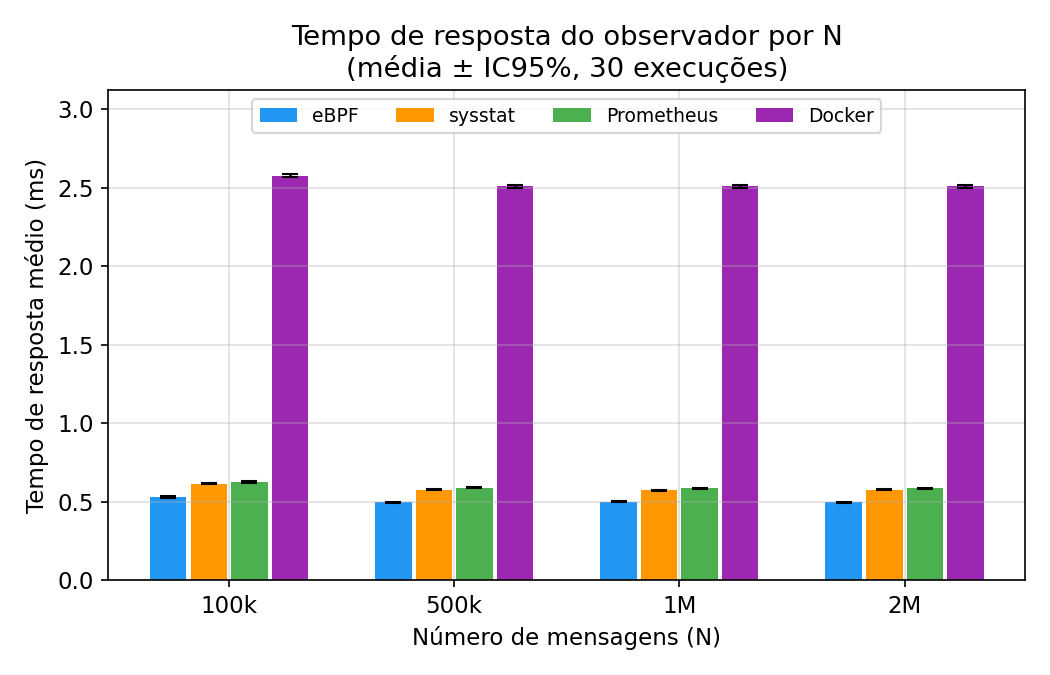
\includegraphics[width=\columnwidth]{tempo_resposta_por_n.png}
\caption{RTT médio do observador por volume de mensagens.}
\label{fig:rtt}
\end{figure}

\begin{figure*}[t]
\centering
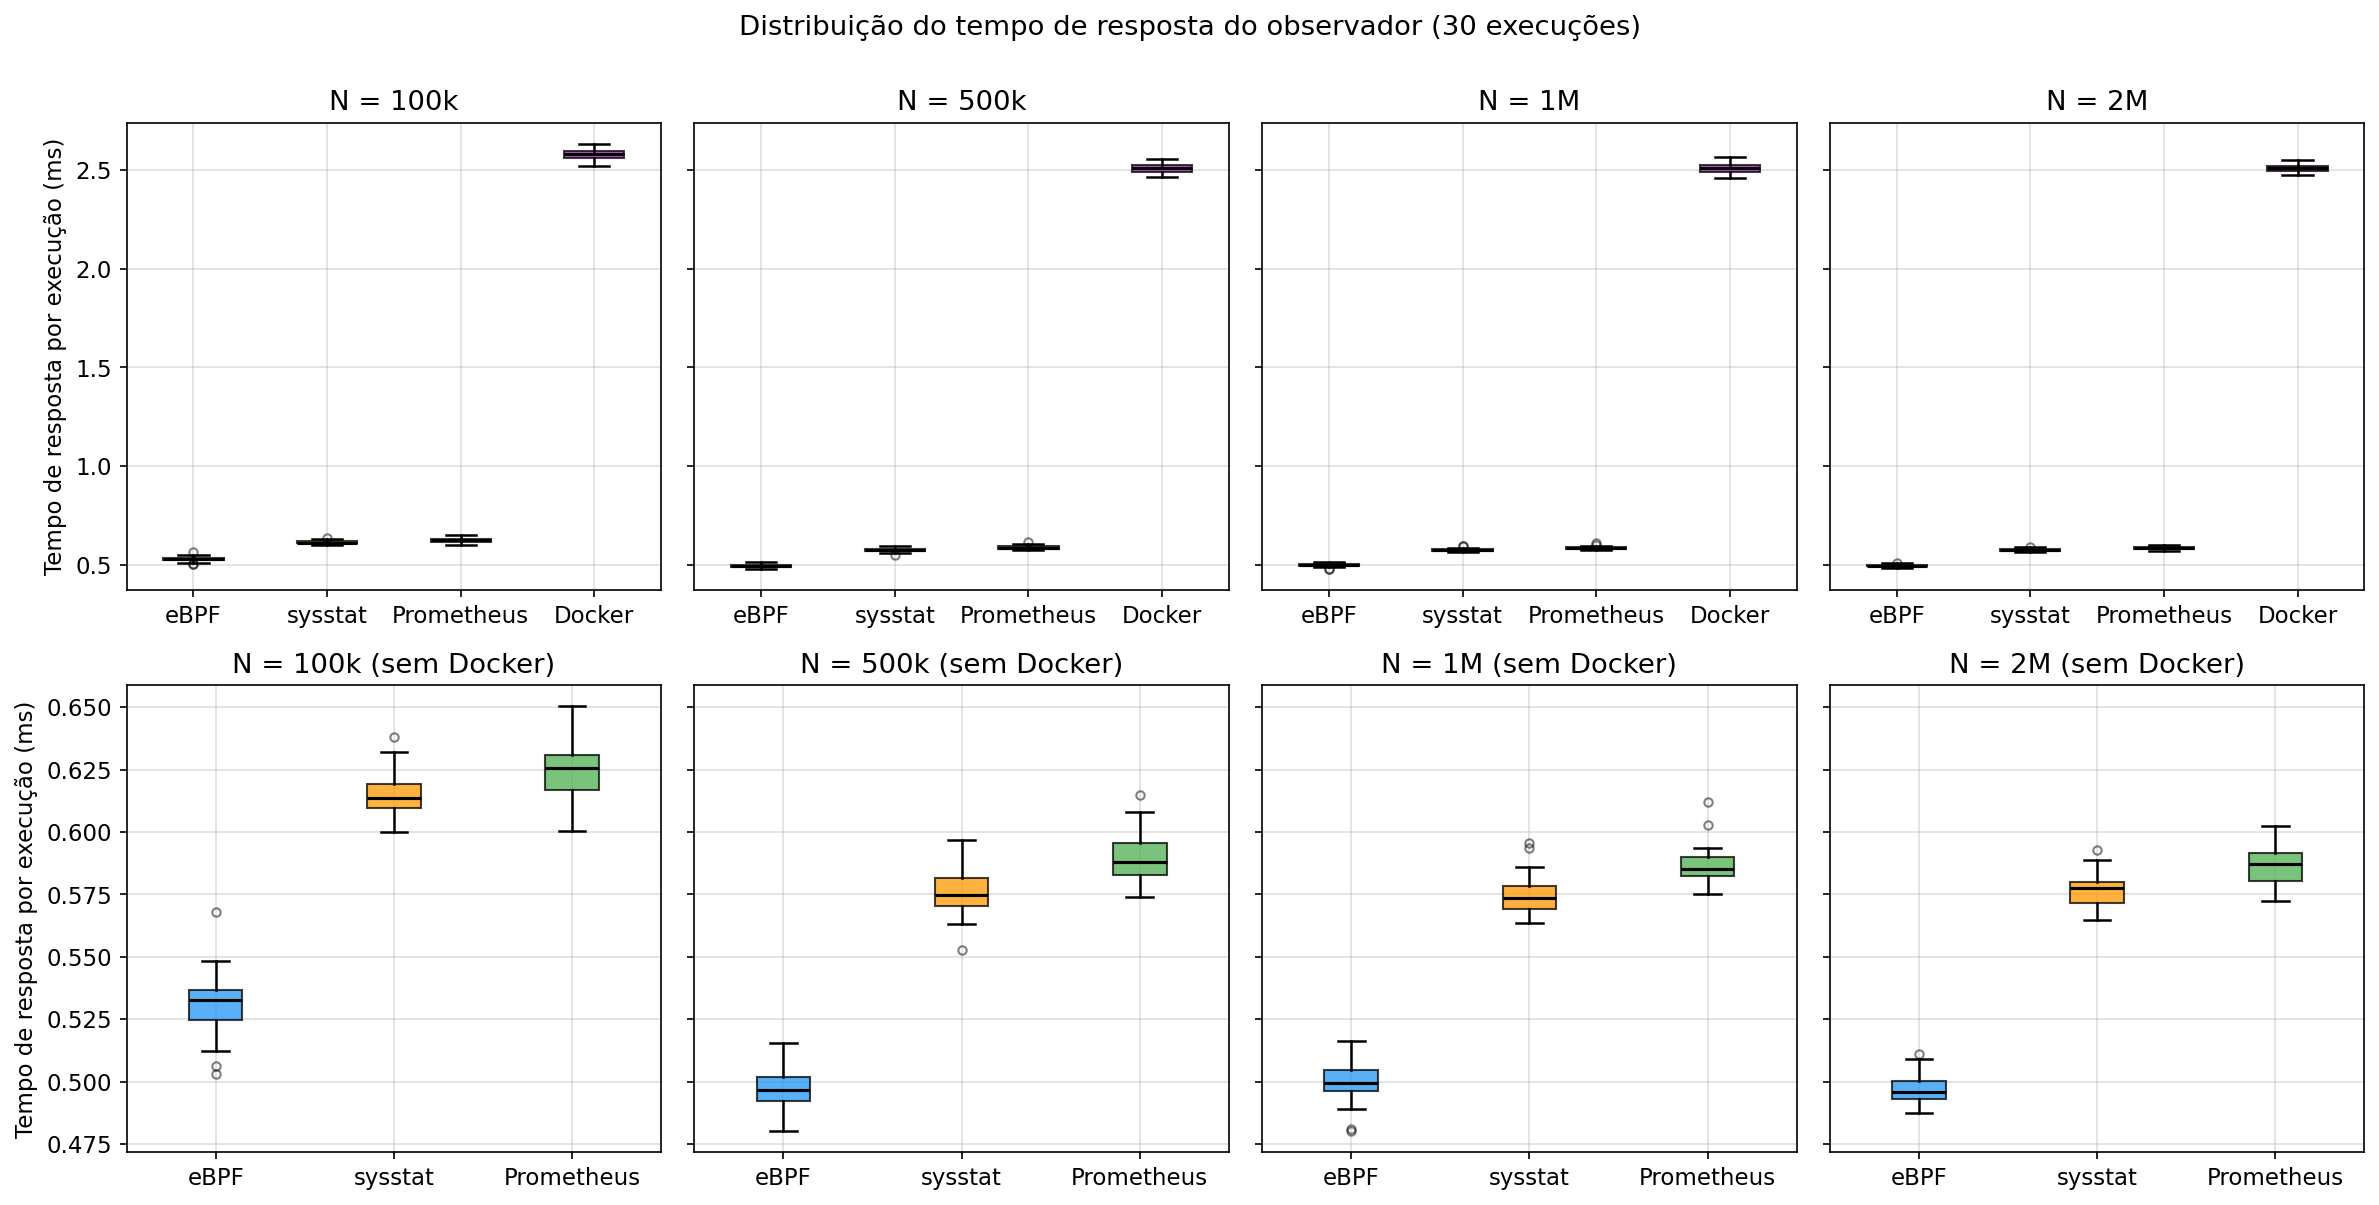
\includegraphics[width=0.85\textwidth]{boxplot_tempo_resposta.png}
\caption{Distribuição do RTT por ferramenta e volume (30 execuções). A linha inferior omite o Docker e amplia o eixo.}
\label{fig:box}
\end{figure*}

\subsection{Por que o Docker é mais lento}
A diferença decorre da interface de coleta, e não da métrica. No Sysstat e no Prometheus, a leitura é local (arquivos de \texttt{/proc} e chamadas do \texttt{psutil}), e no eBPF é a leitura de um contador em memória. No Docker, cada sonda UDP dispara uma cadeia síncrona: o SDK Python monta uma requisição HTTP e a envia pelo \textit{socket} Unix; o \textit{daemon} lê os arquivos do \textit{cgroup}, monta a estrutura completa de estatísticas (CPU por núcleo, memória, rede, E/S) e a serializa em JSON; o SDK decodifica a resposta; e o observador calcula a variação de CPU. Como o observador só responde ao UDP depois dessa cadeia, todo o seu custo integra o RTT.

Um microbenchmark isolado, em outra máquina e com o contêiner ocioso (\texttt{scripts/bench\_docker\_cgroup.py}), mostra a proporção entre as etapas: a chamada \texttt{stats(one\_shot)} do SDK levou de 1,4 a 1,7 ms; uma chamada vazia ao \textit{daemon}, que mede só a ida e volta pela API, de 0,5 a 0,6 ms; e a leitura direta de \texttt{cpu.stat}, \texttt{memory.current} e \texttt{memory.stat} do \textit{cgroup}, de 0,04 a 0,05 ms, cerca de 30 vezes menos. Os cerca de 2 ms que o Docker acrescenta ao RTT na coleta são maiores que a chamada isolada, o que é compatível com a competição por CPU entre o \textit{daemon} e o WAF saturado, mas essa parcela não foi decomposta. Manter a consulta em segundo plano ou guardar o último valor em \textit{cache} reduziria o RTT, mas à custa da atualidade da métrica e em desvantagem para os demais coletores, que leem seus dados na hora da requisição; por isso essas alternativas não foram implementadas.

\subsection{Memória e CPU}
O Sysstat teve o menor consumo de memória (13,6 MB), seguido do eBPF (15,0 MB), do Prometheus (24,7 MB) e do Docker (30,8 MB), sem relação com o volume. A CPU do WAF saturou em torno de 104\% a 110\% de um núcleo a partir de $N=500$ mil, sem diferença prática entre os coletores (em $N=1$ milhão, entre 105,3\% e 106,1\%), o que indica que a escolha do coletor não altera o custo da VNF. A CPU do próprio observador foi muito ruidosa e não sustenta comparação quantitativa. A Figura~\ref{fig:mem} mostra a memória do observador por volume.

\begin{figure}[t]
\centering
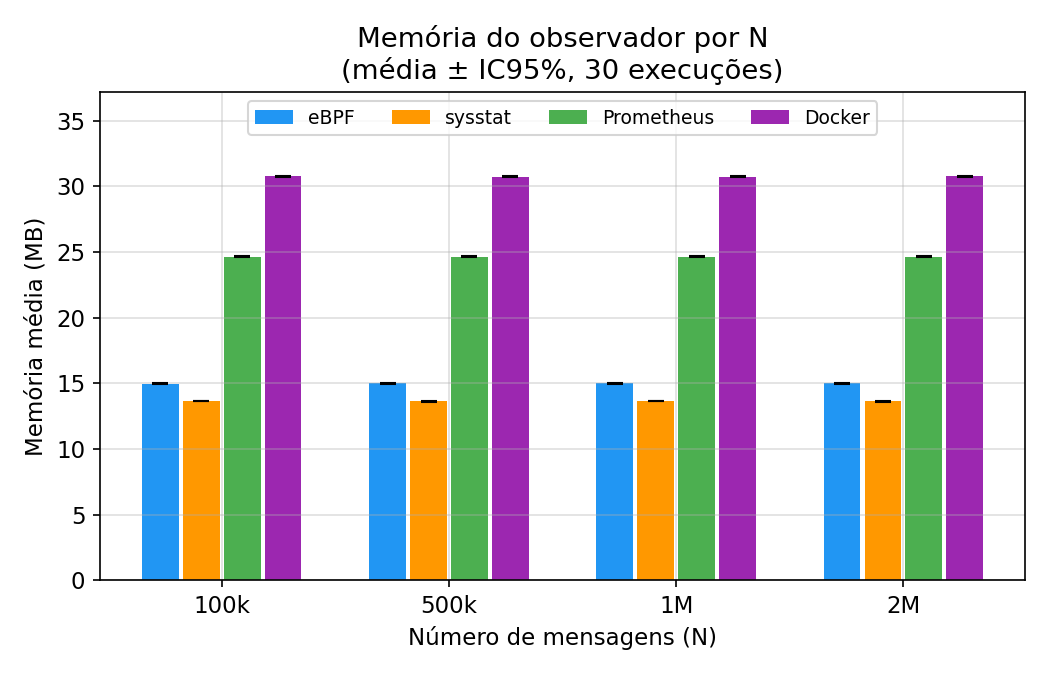
\includegraphics[width=\columnwidth]{memoria_observador.png}
\caption{Memória média do observador por volume de mensagens (média $\pm$ IC95\%, 30 execuções).}
\label{fig:mem}
\end{figure}

\subsection{Análise de sensibilidade da vazão}
Nos volumes maiores, o WAF inspecionou apenas de 62\% a 88\% das mensagens, a uma vazão de cerca de 7 a 8 mil mensagens por segundo, abaixo dos 15\,000 por segundo usados para dimensionar a janela. Em testes com o eBPF e $N=1$ milhão, o limite resultou de dois fatores simultâneos: o processo único do WAF e a leitura dos arquivos de carga pelo cliente. Com o WAF e o cliente em 4 processos e leitura direta, o WAF inspecionou 100\% das mensagens. A bateria completa foi repetida com essa configuração (480 execuções): a ordem entre as ferramentas se manteve e os IC95\% ficaram entre $\pm0{,}004$ e $\pm0{,}011$ ms. O RTT absoluto subiu (Tabela~\ref{tab:sens}), pois os observadores baseados em \texttt{psutil} passam a consultar os quatro processos do WAF a cada sondagem; o Docker, que consulta o contêiner por uma única chamada, subiu pouco. Por isso os valores absolutos da coleta principal, com um processo, são os que se reportam.

\begin{table}[t]
\centering
\caption{RTT médio (ms) em $N=1$ milhão: coleta principal e coleta com inspeção integral (WAF e cliente em 4 processos).}
\label{tab:sens}
\footnotesize
\begin{tabular}{@{}lcccc@{}}
\toprule
 & eBPF & Sysstat & Prometheus & Docker \\
\midrule
Principal (62--88\% inspecionado) & 0,498 & 0,575 & 0,585 & 2,498 \\
Inspeção integral (100\%)         & 0,900 & 1,014 & 1,037 & 2,658 \\
\bottomrule
\end{tabular}
\end{table}

\section{Considerações Finais}
\label{sec:conc}
Os resultados sustentam a hipótese: o eBPF apresentou o menor tempo de resposta em todos os volumes, com diferenças estatisticamente significativas em relação às demais abordagens. A vantagem sobre o Sysstat e o Prometheus é de magnitude moderada (13\% a 15\%, ou cerca de 0,07 a 0,09 ms), ao passo que a API do Docker ficou cinco vezes acima, por causa da cadeia de consulta ao \textit{daemon}. O Sysstat teve o menor consumo de memória, e a escolha do coletor não alterou a CPU do WAF; portanto, a escolha da ferramenta deve ponderar também a complexidade de implementação.

As limitações são o uso de uma única máquina, de um WAF simplificado em Python e de tráfego sintético em \textit{loopback}, de modo que a generalização para outros ambientes não está assegurada, e o fato de a CPU do observador não ter sustentado comparação. Como trabalhos futuros, propõem-se: repetir a coleta do Docker lendo os \textit{cgroups} diretamente (em \texttt{/sys/fs/cgroup/system.slice/}), em vez de usar a biblioteca \texttt{docker}; avaliar um WAF de maior vazão, que inspecione todas as mensagens sem múltiplos processos; e estender a comparação a outras VNFs e a ambientes com mais de um contêiner monitorado.

\bibliographystyle{IEEEtran}
\bibliography{../referencias}

%% 'ieeeaccess.cls' exige \EOD ao fim do documento
\EOD
\end{document}
